\documentclass[12pt]{article}
%\documentclass{acmtog}

\usepackage[english]{babel}
%\usepackage[utf8x]{inputenc}
\usepackage{amsmath}
\usepackage{graphicx}
\usepackage{hyperref}
\usepackage{algorithm2e}


\hypersetup{
colorlinks=false,
pdfborder={0 0 0},
backref=true,
bookmarksnumbered,
pdfstartview={FitH},
citecolor={blue},
linkcolor={blue},
urlcolor={black},
pdfpagemode={UseOutlines}
}

\title{Interactive Hard Shadows Overview}
\author{James Doverspike}

\begin{document}
\maketitle

\begin{abstract}
Visual quality in interactive applications depends on accurate shadowing from light sources. Soft shadows as a result of global illumination are rarely an option due to complexity. This paper analyzes the two popular hard shadowing algorithms of shadow mapping and shadow volumes. 
\end{abstract}

\section{Introduction}

Shadow mapping was first proposed by Williams ~\cite{Williams:1978:CCS:800248.807402} in 1978. It was the first algorithm to use a depth buffer to compute shadows. Later Crow introduced the method of shadow volumes ~\cite{Crow:1977:SAC:563858.563901}. It was not until Doom 3 that Crow's method was implemented in a popular application. Both of these methods are now commonly used in interactive applications. Shadow mapping, however, is more common due to its higher performance.

Both shadowing algorithms generate hard shadows. A hard shadow is a shadow without a penumbra. This is because the algorithms only support point and directional light sources. Area light sources generate soft shadows because points may be partially in shadow. The sampling technique used in shadow mapping, however, gives the illusion of a small penumbra around the shadow even though the lights should only cast perfectly hard shadows.  The shadows from the shadow volume algorithm are binary--a point is either lit or unlit by a given light.

\section{Implementation Details}

Both techniques are written in C++ for Windows using Direct3D 11. The rendering engine is capable of drawing many high-polygon and low-polygon models with multiple non-area light sources at interactive rates. The shadow volumes algorithm generates shadows accurate to a pixel resolution, providing a reference for the visual quality of the shadow mapping algorithm.

\section{Shadow Mapping}

\subsection{Overview}

The shadow algorithm is just a projection from a point light source of the scene onto a plane. The algorithm has two steps: render from the light's position only into the Z-buffer, then render from the eye's position and construct the transformation that maps the coordinates of the eye to the coordinates of the camera. As each point is rendered from the eye's view, it is transformed to the light's view and compared against the Z-buffer depth.
If the depth of the fragment is greater than the Z-buffer depth is not visible to the light source and in shadow.


\begin{algorithm}
\tcc{Generate the depth maps for each light}
\For{every light}
{
	\tcc{These loops run in parallel on the GPU}
	\For{every triangle}
	{
		\For{ every pixel covered by triangle}
		{
			update depth
		}
	}
}
\end{algorithm}

The complexity of the second loop depends on the number of triangles culled. The complexity of the third loop depends on the average number of pixels that a triangle covers. In the worst case, every triangle covers the entire frame and none are culled.
The complexity is then \(O(l*n*r^2)\), where \(l\) is the number of lights, \(n\) is the number of triangles, and \(r^2\) is the resolution.

After the shadow maps are generated there is a single render pass. The fragment shader runs in a loop that computes the Percentage-Closer Filtering coverage for each light. The coverage is used as a normalized weight for the light emitted from the surface.


\subsection{Percentage-Closer Filtering}

The major restraint of shadow mapping is the resolution of the depth map. Since the size of the frustum determines the resolution, casters that are far apart cause the shadow quality to degrade. The tightest frustum must be chosen to maximize sample quality.

Despite shadow mapping being an image-space algorithm, typical sampling techniques do not work with shadow maps because shadow maps store depth and not color. The algorithm does a comparison for each pixel to determine visibility. A shadow map is therefore a two-dimensional array of boolean values indicating whether a given fragment is in shadow. Sampling techniques can then be used on the boolean texture to compute the "coverage" of a neighborhood about a fragment. The resuling value ranges between zero and one.
This value can be used to weight the brightness of the shaded fragment, creating a penumbra at shadow edges.

\begin{algorithm}
result = 0\;
\For{each light}
{
	\tcc{Shade the fragment using the current light}
	color = ComputeColor()\;
	coverage = 0\;
	\tcc{The shadow map is sampled in a window centered at the fragment}
	\For{window width}
	{
		\For{window height}
		{
			\tcc{The fragment's depth is compared to the shadow map depth. The result is either 0 or 1.}
			coverage = coverage + shadowMap.SampleCompare(x, y, depth)\;
		}
	}
	coverage = coverage / (width * height)\;
	result = result + coverage * color\;
}
\KwRet{result}
\end{algorithm}

This is percentage-closer filtering. The weight or "coverage" at a given fragment denotes whether a fragment is near a shadow border. Instead of having a jagged stair-stepping pattern at shadow edges due to resolution constraints, PCF creates a soft shadow.
This effectively anti-aliases the shadow map. Note that a soft shadow will result from non-area lights.

\begin{figure}
\centering
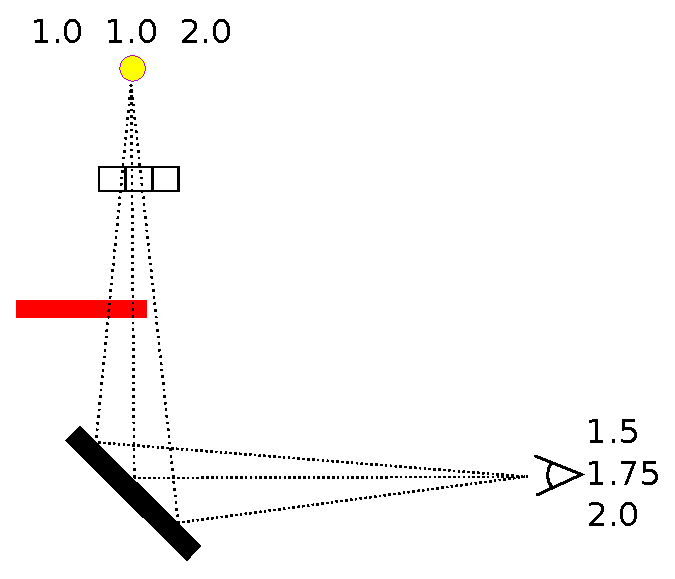
\includegraphics[scale=0.5]{depth2.eps}
\caption{\label{fig:depth} Depth values of depth map and current fragments.}
\end{figure}


\begin{figure}
\centering
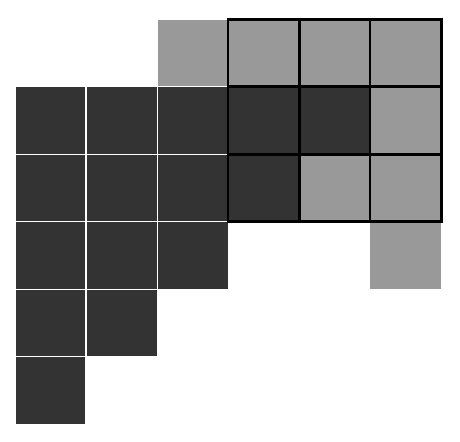
\includegraphics[scale=0.5]{pcf.eps}
\caption{\label{fig:pcf} A 3x3 PCF filter window. The weight of the fragment of the lighter triangle is 6/9.}
\end{figure}

Figure \ref{fig:depth} shows the depth values from the light and the eye for three pixels. Note that the rays traced from the scene back to the light do not land on at depth map centers. The three depths from the depth map using linear interpolation would be 1.0, 1.0, and 1.7. Comparing these values against the depths from the eye (1.5, 1.75, and 2.0) tells us that all three points are in shadow because the depth map values are closer.
Obviously the third value should not be in shadow. The problem with linear interpolation is that it averages depths between two objects, creating a depth value of 1.7 which is somewhere between the depths of the two objects.
PCF would instead compare the eye depth of 2.0 to the depth map values of 1.0 and 2.0. The first value is in shadow and the second is not in shadow. This gives a coverage of 0.5.
Since the pixel is close to the edge of a shadow it will be partially in shadow.

Figure \ref{fig:pcf} shows a 3x3 sample window on a depth map containing two triangles. The darker triangle is significantly closer than the lighter one. The pixel in the center of the window of the lighter fragment is the one being shaded. If we use a simple PCF averaging filter then the coverage is 6/9 because six fragments are covered by a depth near the current sample and three are much closer. Three of the samples are in shadow because the darker triangle overlaps the lighter one.

\subsection{Shadow Silhouette Maps}

Shadow mapping quality can be improved significantly through the use of Shadow silhouette maps \cite{Sen:2003:SSM:882262.882301}. Shadow silhouette maps store the silhouette edges as well as the depth so that depth lookups become piecewise linear instead of piecewise constant.

\subsection{Implementation}

A shadow map is generated for each light. Choosing a frustum by which to construct the depth map is done using a heuristic that ensures the frustum contains all of the casters. There is one render pass and l depth passes per frame, where l is the number of lights. The resolution of the depth buffer is the same as the frame buffer. Each fragment uses 16 samples of the shadow map to determine coverage, per light.

\subsection{Analysis}

Because shadow mapping is an image-space algorithm, the complexity of increasing the quality of the image corresponds to the square of the resolution \cite{Williams:1978:CCS:800248.807402}.
The complexity of generating and sampling the shadow map depends mostly on the resolution of the depth buffer. Increasing the complexity of the geometry only affects shadow map generation.
Generating the depth map has \(O(n*r^{2}) = O(r^{2})\) complexity, where n is the number of polygons and r is the resolution.
In practice, n and r are similar values such that increasing either the resolution or the complexity of the scene both affect the performance. However, depth passes are considered almost insignificant compared to shading passes and the two-sided stencil pass from shadow volumes. 

\section{Shadow Volumes}

\subsection{Overview}

The method of shadow volumes is a rasterization technique for generating hard shadows. Due to water-tight geometry, "a version of the Jordan curve theorem leads to the conclusion that shadows occur at pixels with non-zero stencil buffer entries" \cite{Sen:2003:SSM:882262.882301}.
The algorithm determines whether a point is in shadow based on a count of the number of polygons intersected by tracing a ray from the eye to the point. The polygons that are rasterized are "shadow polygons": polygons extruded from the silhouette of shadow-casting geometry.
When intersecting the ray with the shadow polygons during rasterization a counter is incremented if the polygon is front-facing and decremented if it is back-facing. If the count is zero the point is not within any shadow geometry. Either there is no shadow geometry between the eye and the point or the ray passed entirely through one or more shadow volumes. A positive count implies that a volume was entered but not exited, meaning that the point lies within the volume and in shadow. Since all shadow volumes are water-tight, a negative count implies that the eye is within at least one volume that the ray exited without entering.

The count of every pixel is stored in the stencil buffer. This may be done in two passes with a single-sided stencil buffer or one with a two-sided stencil buffer (one that allows front-facing and back-facing values fragments to contribute).

The algorithm consists of three passes: the depth pass, the stencil buffer pass, and the render pass. The first pass computes the Z-buffer that corresponds to geometry in the scene.
The second pass generates and rasterizes shadow volumes based on silhouette edges. The third pass renders the frame and accumulates the frame with the previous frames.

\begin{algorithm}
depth pass\;
\For{every light}
{
	stencil pass\;
	render pass\;
	add frame\;
}
\end{algorithm}

The stencil pass is equivalent to the depth pass in complexity. However, the depth pass is substantially faster because more geometry can be culled. Back-facing shadow polygons need to be rasterized into the stencil buffer. The stencil pass also includes shadow polygon generation from silhouette edges. The render pass is also the same in complexity as the depth pass but slower because each fragment must be shaded.

\subsection{Z-pass and Z-fail}

The Z-pass shadow volumes algorithm rasterizes all of the shadow volumes closer than the depth buffer. The depth of the scene is first generated from the depth pass. Then the shadow geometry is rasterized and the stencil buffer count is changed only if the shadow volume fragment is closer than the scene fragment according to the depth buffer.
It is called Z-pass because only shadow volume fragments that pass the depth test are accumulated in the stencil buffer.

The Z-fail shadow volumes algorithm differs from Z-pass by the depth test function. Shadow volume fragments accumulate in the stencil buffer only if the fragments fail the depth test. This corresponds to rasterizing all of the geometry behind the scene instead of in front of it.

The key difference between the two methods is that Z-pass generates inverted shadows when the eye is within a shadow volume. If a ray is traced from the eye to the scene when the light is in shadow, the count will be off by one because the ray never entered the volume. The count must start at the proper value instead of zero.
A ray can be traced from the light (with a point light) or from infinity (with a directional light) to the eye to compute the initial offset.
This is very computationally expensive because it requires another pass over the geometry.

The other major difference between Z-pass and Z-fail is performance. According to \cite{Sen:2003:SSM:882262.882301}, Z-fail can be up to 80\% slower than Z-pass.

\subsection{Implementation}

The shadow volumes are generated on the GPU per-frame by the geometry shader. Silhouette edges are detected by a difference in sign between the direction of adjacent faces with respect to the eye direction.
A face is front-facing if the dot product of the face and the eye direction is negative. A silhouette edge is therefore the edge shared by two faces where one is front-facing and the other is back-facing.

Every front-facing polygon corresponds to a front cap and a back cap. The front cap is the same position of the face and the back cap is the position projected to infinity in the direction of the light. Directional light sources create front and back caps of the same size and point light sources grow the back caps.

Silhouette edges generate a side quad that connects a front cap and a back cap.

\subsection{Analysis}

The shadow volumes algorithm is geometry-bound. Each light requires an entire stencil pass because the shadow volumes depend on the direction of the light.
Every frame requires one depth pass, one render pass, and l stencil passes where l is the number of lights. Shadow volume generation and rasterization is dominated by the front and back caps because the caps are created from a two-dimensional patch of the surface whereas the sides are created from a one-dimensional slice through the geometry.

\section{Results}

See Table~\ref{tab:widgets}

\begin{figure}
\centering
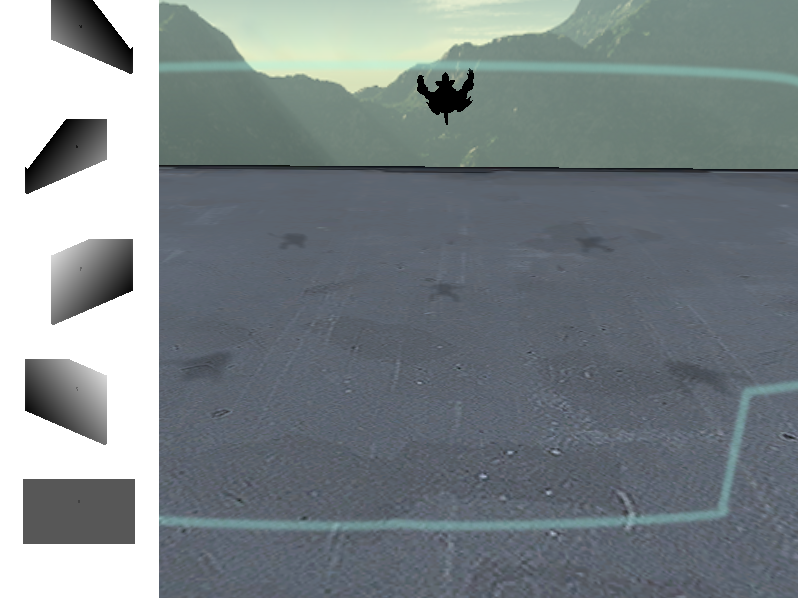
\includegraphics[scale=0.5]{ArmadilloMaps.png}
\caption{\label{fig:mapping} Shadow mapping with 5 lights. The shadow maps are on the left.}
\end{figure}

\begin{figure}
\centering
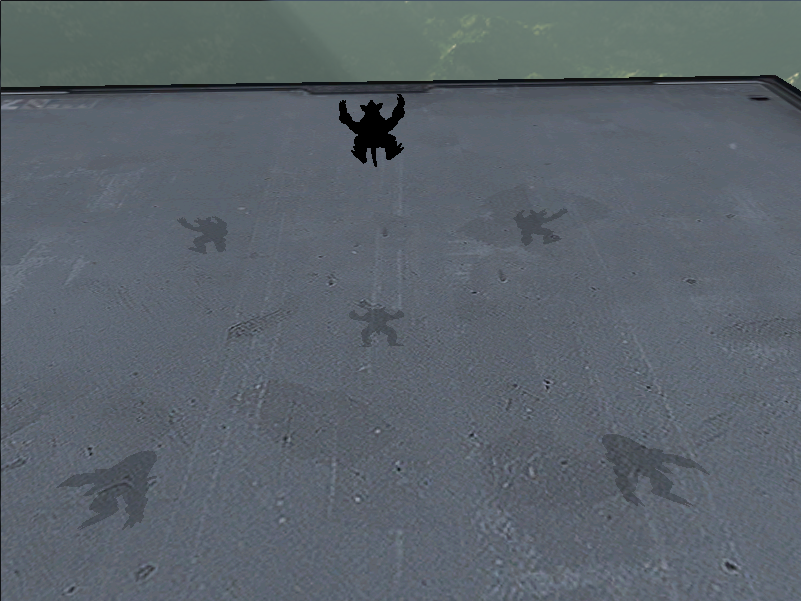
\includegraphics[scale=0.5]{ArmadilloVolumes.png}
\caption{\label{fig:volumes} Shadow volumes with 5 lights.}
\end{figure}

\begin{table}
\centering
\begin{tabular}{|l|c|r|}
\hline
Lights & Shadow Mapping & Shadow Volumes \\\hline
5 & 168.9 & 28.5 \\
4 & 210.2 & 36.3 \\
3 & 276.9 & 57.6 \\
2 & 379.7 & 87.4 \\
1 & 378.5 & 179.9 \\
\hline
\end{tabular}
\caption{\label{tab:widgets} Average frames per second of the 345,944 triangle Armadillo model}
\end{table}

\section{Future Work}

Silhouette mapping and Z-Pass using a triangle intersection compute shader have yet to be completed. The next logical step from hard shadows is either simulated soft shadows by filtering the shadow map or real soft shadows as a result of global illumination.
\cite{Dachsbacher:2005:RSM:1053427.1053460} uses shadow maps to render indirect lighting.

\bibliographystyle{plain}
\bibliography{references}

\end{document}
